\documentclass[border=10pt]{standalone}

\usepackage{tikz}
\usepackage{tikzsymbols}
\usetikzlibrary{calc,patterns,shapes.geometric}

\def\centerarc[#1](#2)(#3:#4:#5){\draw[#1] ($(#2)+({#5*cos(#3)},{#5*sin(#3)})$) arc (#3:#4:#5);}

\begin{document}
	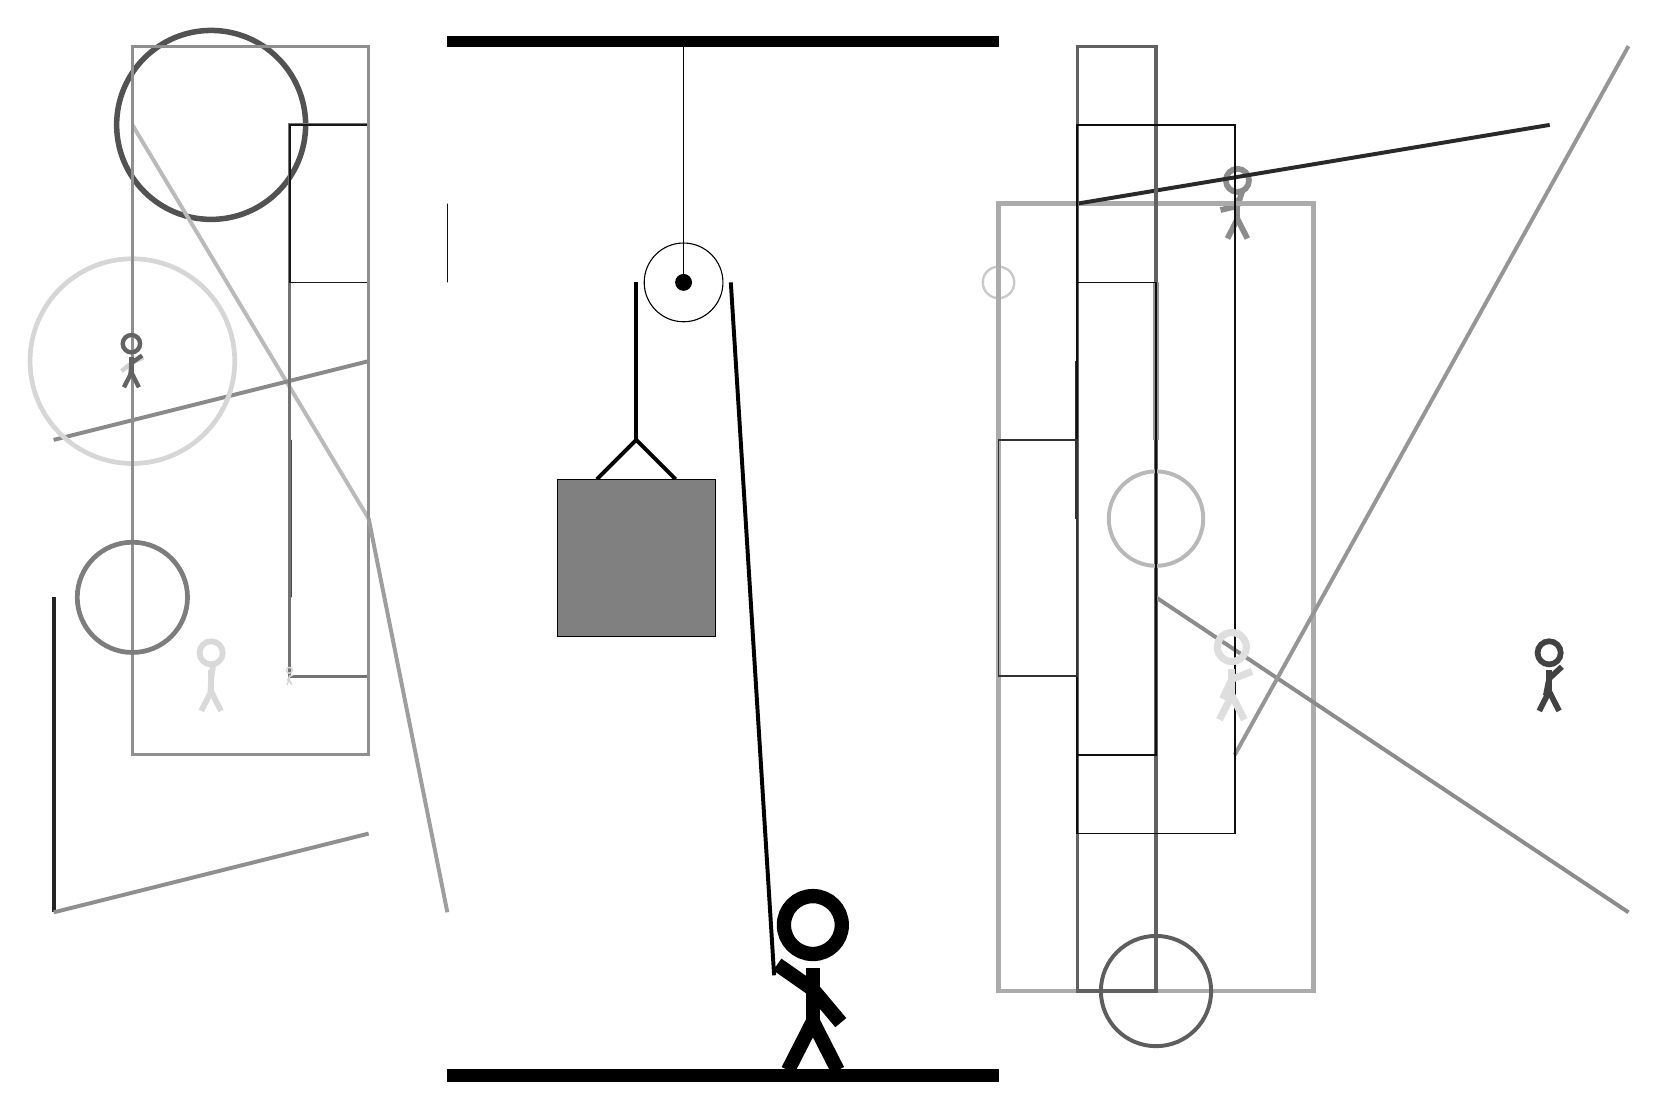
\begin{tikzpicture}
		%%%%% START %%%%%
		
		\draw[fill=black] (-2, 10) rectangle (5, 10.125);
		
		\draw (1, 7) circle (0.5);
		\draw[fill=black] (1, 7) circle (0.1);
		\draw (1, 10) -- (1, 7);
		
		\draw[line width=0.5mm] (-0.1, 4.5) -- (0.4, 5.0) -- (0.9, 4.5);
		\draw[fill=black!50] (-0.6, 4.5) rectangle (1.4, 2.5);
		
		\draw [line width=0.7mm, color=black!68](-5, 9) circle (1.2);
		
		\draw[line width=0.5mm, color=black!86](-7, -1) -- (-7, 3);
		\draw [line width=0.7mm, color=black!52](-2, -2) circle (0.0);
		\draw [line width=0.3mm, color=black!21](5, 7) circle (0.2);
		\node[line width=0.6mm, color=black!45] at (8, 8) {\Strichmaxerl[4][13][72]};
		
		\node[line width=0.4mm, color=black!18] at (-6, 6) {\Strichmaxerl[3][39][25]};
		\draw[line width=0.6mm, color=black!71] (-4, 5) rectangle (-4, 3);
		
		\draw[line width=0.5mm, color=black!27](-3, 4) -- (-6, 9);
		\draw[line width=0.6mm, color=black!33] (5, 8) rectangle (9, -2);
		
		\draw[line width=0.5mm, color=black!44](-3, 0) -- (-7, -1);
		\draw[line width=0.5mm, color=black!46](-3, 6) -- (-7, 5);
		\draw[line width=0.4mm, color=black!55] (-3, 9) rectangle (-4, 2);
		\draw[line width=0.5mm, color=black!84](6, 8) -- (12, 9);
		
		\draw[line width=0.5mm, color=black!81](6, 6) -- (6, 4);
		\draw[line width=0.4mm, color=black!62] (6, 10) rectangle (7, -2);
		\draw[line width=0.5mm, color=black!45](7, 3) -- (13, -1);
		
		\node[line width=0.6mm, color=black!17] at (-4, 2) {\Strichmaxerl[1][64][26]};
		\draw [line width=0.5mm, color=black!28](7, 4) circle (0.6);
		\draw[line width=0.2mm, color=black!91] (-3, 9) rectangle (-4, 7);
		
		\node[line width=0.6mm, color=black!15] at (-5, 2) {\Strichmaxerl[4][87][81]};
		\draw [line width=0.6mm, color=black!16](-6, 6) circle (1.3);
		\node[line width=0.7mm, color=black!74] at (12, 2) {\Strichmaxerl[4][79][43]};
		
		\draw[line width=0.7mm, color=black!41] (7, 5) rectangle (7, 7);
		\draw[line width=0.5mm, color=black!41](8, 1) -- (13, 10);
		\draw[line width=0.2mm, color=black!95] (6, 0) rectangle (8, 9);
		
		\draw[line width=0.2mm, color=black!94] (6, 7) rectangle (7, 1);
		\draw[line width=0.2mm, color=black!80] (5, 5) rectangle (6, 2);
		\draw[line width=0.4mm, color=black!44] (-3, 1) rectangle (-6, 10);
		\node[line width=0.6mm, color=black!13] at (8, 2) {\Strichmaxerl[5][65][21]};
		
		\node[line width=0.3mm, color=black!61] at (-6, 6) {\Strichmaxerl[3][85][35]};
		\draw [line width=0.5mm, color=black!63](7, -2) circle (0.7);
		
		\draw[line width=0.5mm, color=black!38](-2, -1) -- (-3, 4);
		\draw[line width=0.2mm, color=black!93] (-2, 8) rectangle (-2, 7);
		\draw [line width=0.6mm, color=black!51](-6, 3) circle (0.7);
		
		\draw[line width=0.5mm] (0.4, 7) -- (0.4, 5.0);
		\centerarc[line width=0.5mm](1, 7)(0:180:0.6);
		\draw[line width=0.5mm](1.6, 7) -- (2.15, -1.8);
		
		\node at (2.6, -1.9) {\Strichmaxerl[10][-35][-50]};
		
		\draw[fill=black] (-2, -3) rectangle (5, -3.15);
		
		%%%%% END %%%%%
	\end{tikzpicture}
\end{document}